\section{Application to sensor design}
\label{sec:design}

\subsection{An alignment error in the design analysis, and its consequence}
The Task~8 design analysis defines candidate sensor cores as short motifs and scores them as eight-residue windows. Three of the four cores, PRSLSGLK, PLGLAGQS and PLGVALAA, are motifs whose scissile bond lies after the \emph{third} residue (Pro-Arg-Ser$\downarrow$Leu, Pro-Leu-Gly$\downarrow$Leu; $\pos{3}=\mathrm{Pro}$ and $\prm{1}=\mathrm{Leu}$, matching the consensus of Kridel et al.). Read as a P4--P4$'$ window, whose bond is after the fourth character, every residue is shifted one position from its intended subsite: for PRSLSGLK the window has $\pos{2}=\mathrm{S}$ and $\prm{1}=\mathrm{S}$ instead of $\pos{2}=\mathrm{R}$ and $\prm{1}=\mathrm{L}$. The design plan itself states the intended features as ``P2 = Arg, P1$'$ = Leu, P2$'$ = Ser'', which the shifted window does not encode.

The model responded correctly to the wrong input: PRSLSGLK scored at the $7$th percentile for MMP-9. Scored as the gapped window \texttt{-PRSLSGL} with the bond after the third residue, it scores at the $100$th percentile (and at the top for MMP-2 and MMP-8, Table~\ref{tab:cand}). The correction also changes a design conclusion. The $3\times3$ specificity matrix of the MMP-2/MMP-9/NE design analysis has condition number $61.7$ with the shifted windows (``poorly conditioned, pivot to a two-plex'' by the analysis's own rule) and $16.1$ with the corrected windows (``marginal''). The corrected matrix still shows that the MMP-2 and MMP-9 candidates are not separable by score, as the selectivity results of Section~\ref{sec:res-sel} predict.

\begin{table}[!htbp]
\centering\small\begin{tabular}{@{}llllcc@{}}\toprule
Candidate & Core & Scored window & Target & Margin (3-plex) & Pool percentile \\\midrule
Cand1 MMP9 & \texttt{PRSLSGLK} & \texttt{-PRSLSGL} & MMP-9 & -0.00 & 16 \\
Cand2 MMP2 & \texttt{PLGLAGQS} & \texttt{-PLGLAGQ} & MMP-2 & -0.00 & 0 \\
Cand4 NE & \texttt{AAPVSGIG} & \texttt{AAPVSGIG} & NE & +0.51 & 26 \\
Cand3 MMP2b & \texttt{PLGVALAA} & \texttt{-PLGVALA} & MMP-2 & -0.04 & 0 \\
\bottomrule\end{tabular}

\caption{Task~8 candidates scored in the MMP-2/MMP-9/NE panel with correctly aligned, gapped windows. ``Pool percentile'' is the percentile of the margin within the PSSM top-3 enumeration pool for the target (same gap pattern).}
\label{tab:design}
\end{table}

\subsection{Candidate landscape in the wound panel}
Figure~\ref{fig:cand} and Table~\ref{tab:cand} rank candidates in the five-protease wound panel (MMP-2, MMP-8, MMP-9, NE, LasB). The pool combines $150{,}000$ random windows with the PSSM top-3 enumerations of each target, filtered by the device constraints of the Task~8 design (no Cys or Trp, net charge $-1$ to $+2$, no Pro-Pro, core mass $600$--$1100$~Da). Three observations matter.

\begin{enumerate}
\item \textbf{The best-scoring sequences are model optima, not recommendations.} They are extreme points of a search over a random pool, far from any training window, and their scores extrapolate. They are hypotheses for wet-lab testing.
\item \textbf{The MMP-family reference cores have margin $\approx 0$.} The corrected MMP-9 cores (IPRTLTA$-$ and $-$PRSLSGL) score at the top for MMP-2, MMP-8 and MMP-9 alike, so no selectivity among MMPs is predicted. (Kridel et al.\ found A11 to be $2.9$-fold and $9.6$-fold more active on MMP-9 than on MMP-13 and MMP-7; neither is in our panel, so this cannot be tested here.)
\item \textbf{The panel changes the answer.} AAPVSGIG has margin $+0.51$ in the three-protease panel but $0.00$ in the wound panel, because the LasB model, trained largely on Gly/Ala/Pro-rich elastin sequence, scores it at the $99$th percentile. Whether LasB actually cleaves AAPV-type sites is not something these data can settle.
\end{enumerate}

\begin{figure}[!htbp]
\centering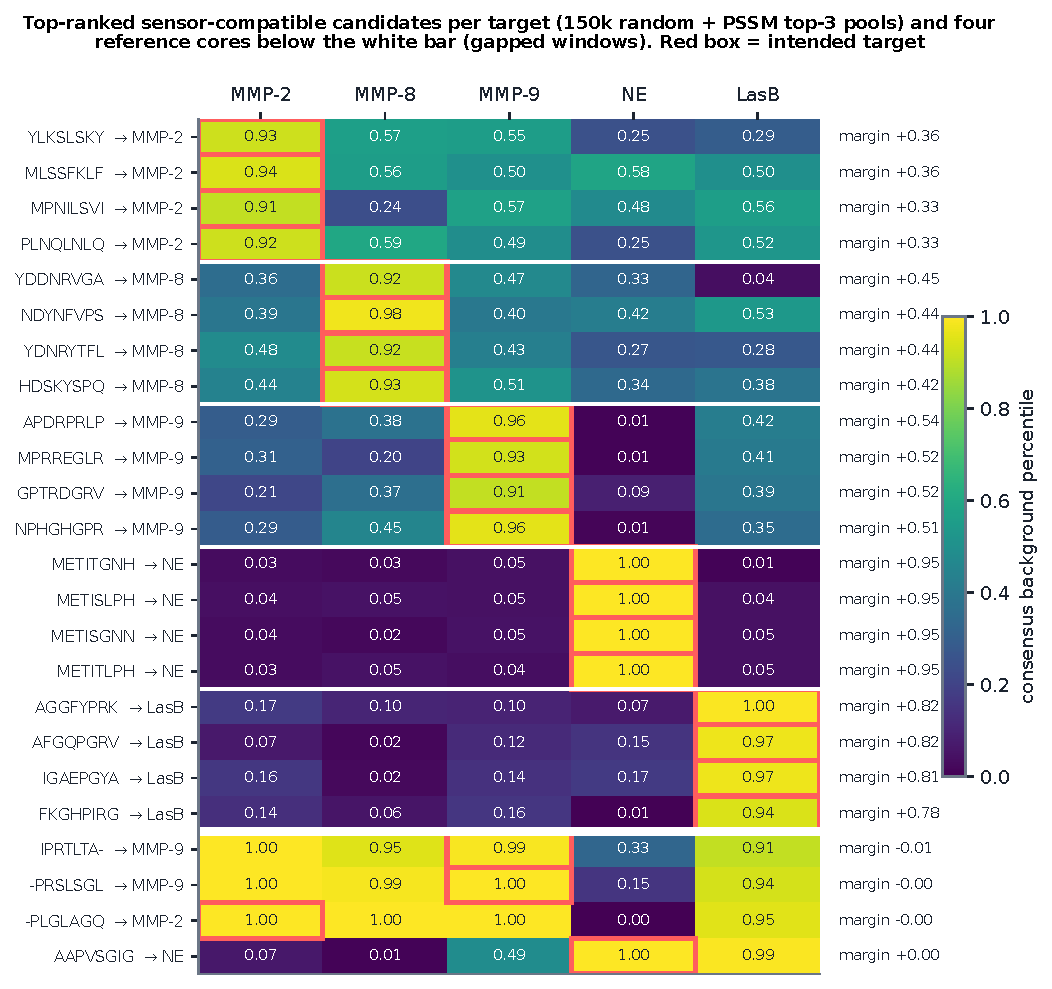
\includegraphics[width=0.85\textwidth]{figures/F17_candidate_landscape.pdf}
\caption{Consensus background percentiles of the four highest-margin sensor-compatible candidates for each target (above the white bar) and of four reference cores (below), across the five wound-panel proteases. Red boxes mark the intended target; margins are listed on the right. Reference cores are scored as gapped windows.}
\label{fig:cand}
\end{figure}

\begin{table}[!htbp]
\centering\small\begin{tabular}{@{}llccccc c@{}}\toprule
Window & Target & MMP-2 & MMP-8 & MMP-9 & NE & LasB & Margin \\\midrule
\texttt{YLKSLSKY} & MMP-2 & 0.93 & 0.57 & 0.55 & 0.25 & 0.29 & +0.36 \\
\texttt{MLSSFKLF} & MMP-2 & 0.94 & 0.56 & 0.50 & 0.58 & 0.50 & +0.36 \\
\texttt{MPNILSVI} & MMP-2 & 0.91 & 0.24 & 0.57 & 0.48 & 0.56 & +0.33 \\
\texttt{PLNQLNLQ} & MMP-2 & 0.92 & 0.59 & 0.49 & 0.25 & 0.52 & +0.33 \\
\texttt{YDDNRVGA} & MMP-8 & 0.36 & 0.92 & 0.47 & 0.33 & 0.04 & +0.45 \\
\texttt{NDYNFVPS} & MMP-8 & 0.39 & 0.98 & 0.40 & 0.42 & 0.53 & +0.44 \\
\texttt{YDNRYTFL} & MMP-8 & 0.48 & 0.92 & 0.43 & 0.27 & 0.28 & +0.44 \\
\texttt{HDSKYSPQ} & MMP-8 & 0.44 & 0.93 & 0.51 & 0.34 & 0.38 & +0.42 \\
\texttt{APDRPRLP} & MMP-9 & 0.29 & 0.38 & 0.96 & 0.01 & 0.42 & +0.54 \\
\texttt{MPRREGLR} & MMP-9 & 0.31 & 0.20 & 0.93 & 0.01 & 0.41 & +0.52 \\
\texttt{GPTRDGRV} & MMP-9 & 0.21 & 0.37 & 0.91 & 0.09 & 0.39 & +0.52 \\
\texttt{NPHGHGPR} & MMP-9 & 0.29 & 0.45 & 0.96 & 0.01 & 0.35 & +0.51 \\
\texttt{METITGNH} & Neutrophil elastase & 0.03 & 0.03 & 0.05 & 1.00 & 0.01 & +0.95 \\
\texttt{METISLPH} & Neutrophil elastase & 0.04 & 0.05 & 0.05 & 1.00 & 0.04 & +0.95 \\
\texttt{METISGNN} & Neutrophil elastase & 0.04 & 0.02 & 0.05 & 1.00 & 0.05 & +0.95 \\
\texttt{METITLPH} & Neutrophil elastase & 0.03 & 0.05 & 0.04 & 1.00 & 0.05 & +0.95 \\
\texttt{AGGFYPRK} & LasB & 0.17 & 0.10 & 0.10 & 0.07 & 1.00 & +0.82 \\
\texttt{AFGQPGRV} & LasB & 0.07 & 0.02 & 0.12 & 0.15 & 0.97 & +0.82 \\
\texttt{IGAEPGYA} & LasB & 0.16 & 0.02 & 0.14 & 0.17 & 0.97 & +0.81 \\
\texttt{FKGHPIRG} & LasB & 0.14 & 0.06 & 0.16 & 0.01 & 0.94 & +0.78 \\
\midrule
\texttt{IPRTLTA-} & MMP-9 & 1.00 & 0.95 & 0.99 & 0.33 & 0.91 & -0.01 \\
\texttt{-PRSLSGL} & MMP-9 & 1.00 & 0.99 & 1.00 & 0.15 & 0.94 & -0.00 \\
\texttt{-PLGLAGQ} & MMP-2 & 1.00 & 1.00 & 1.00 & 0.00 & 0.95 & -0.00 \\
\texttt{AAPVSGIG} & Neutrophil elastase & 0.07 & 0.01 & 0.49 & 1.00 & 0.99 & +0.00 \\
\bottomrule\end{tabular}

\caption{Consensus percentiles and specificity margin for the candidates of Figure~\ref{fig:cand}.}
\label{tab:cand}
\end{table}

\subsection{What each position contributes}
The scan in Figure~\ref{fig:scan} scores every single-residue substitution of IPRTLTA$-$ (the A11 core). Panel~(a) shows the change in the MMP-9 logistic-regression log-odds, which does not saturate; panel~(b) shows the change in specificity margin, which is near zero for most substitutions because the wild-type is already at the top of the MMP percentile scale. Substitutions at $\pos{3}$ are the most damaging (any replacement of Pro costs roughly $1$ to $2.5$ log-odds units), a change of Thr to Arg or Lys at $\pos{1}$ raises the score (consistent with the measured effect of A11m1), and $\prm{1}$ is comparatively tolerant in this model, which is the same underestimation seen for A11m2.

\begin{figure}[!htbp]
\centering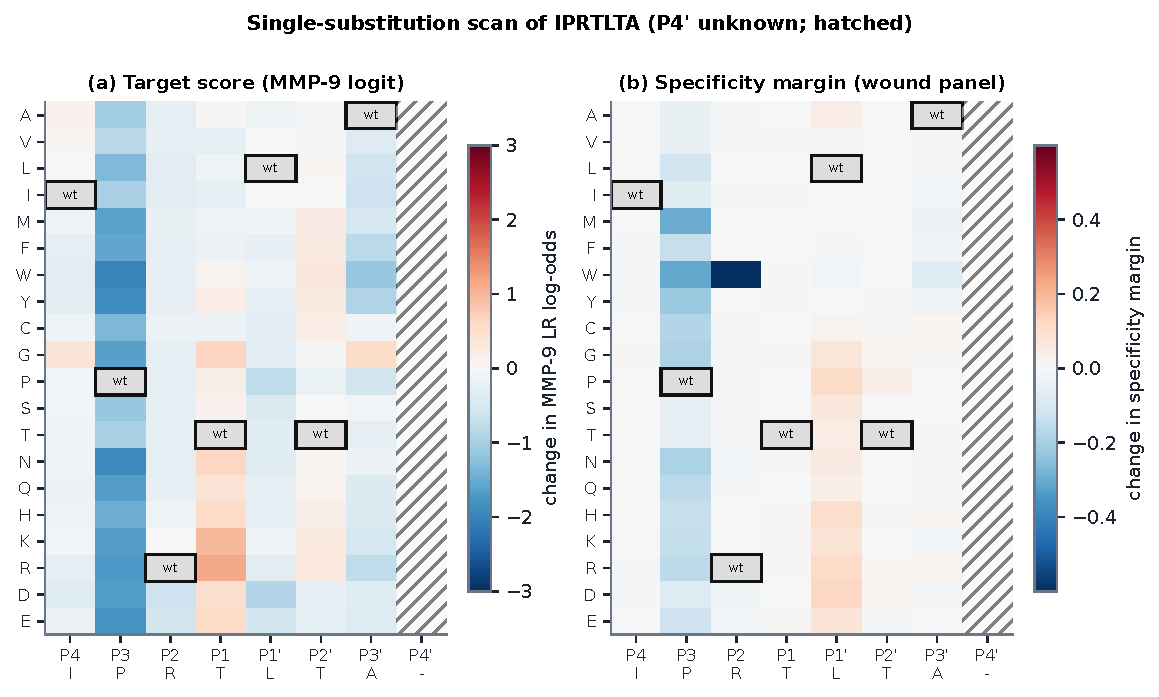
\includegraphics[width=\textwidth]{figures/F18_mutation_scan.pdf}
\caption{Single-substitution scan of the A11 core. \textbf{(a)} Change in MMP-9 logistic-regression log-odds. \textbf{(b)} Change in specificity margin in the wound panel.}
\label{fig:scan}
\end{figure}
